% !TeX root = ../tesi.tex

\chapter{Oltre la conversazione testuale}

Discuto le ragioni per cui Halue ha proposto questo \emph{stage} e per cui io l’ho scelto. Tratto
il ruolo degli \emph{stage} in azienda, il problema che il progetto affronta, il suo posto nella
strategia di Halue, gli obiettivi e i vincoli fissati dal piano di lavoro e le mie motivazioni.

% !TeX root = ../../tesi.tex

\section{Il ruolo degli \emph{stage} nella strategia aziendale}
\label{sec:stage-strategia}

Halue ospita in media tre o quattro \emph{stage} all’anno. Gli stagisti provengono soprattutto
dall’Università di Padova, dai corsi di laurea triennale e magistrale, e alcuni degli \emph{stage}
che hanno preceduto il mio riguardavano già l’intelligenza artificiale. L’azienda attribuisce a
queste esperienze due scopi:

\begin{itemize}
	\item svolgere ricerca e sviluppo su temi che i progetti per i clienti non lasciano il tempo di
	esplorare;
	\item conoscere persone da inserire nel \emph{team}, valutando al termine di ogni percorso la
	possibilità di proseguire la collaborazione con lo stagista.
\end{itemize}

Il primo scopo spiega la forma che gli \emph{stage} assumono. Uno stagista lavora a tempo pieno su
un solo tema per circa due mesi, da 300 a 320 ore lavorative, con una continuità che i dipendenti
non hanno, perché l’azienda li ripartisce ogni mese tra più clienti
(\secref{sec:organizzazione-halue}). Halue affida quindi agli stagisti temi nuovi, su cui non ha
ancora un’esperienza consolidata, e un \emph{tutor} che li segue ogni giorno. Il secondo scopo
spiega perché lo stagista partecipa ai momenti di coordinamento del \emph{team} e ne adotta gli
strumenti, dato che l’azienda valuta il suo modo di lavorare oltre ai risultati che produce.

Ogni \emph{stage} si inserisce in un percorso che lo precede e lo segue. Il tema nasce da
un’esigenza interna oppure dall’interesse che può avere per un laureando in informatica, e nel mio
caso da entrambi, come illustro nella \secref{sec:obiettivi}. Al termine lo stagista presenta il
lavoro a tutto il \emph{team} e partecipa a una retrospettiva, la stessa pratica con cui Halue
chiude gli \emph{sprint} e i progetti per i clienti. Il lavoro può quindi avere due esiti:

\begin{itemize}
	\item l’azienda lo archivia come base di conoscenza sul tema;
	\item l’azienda lo rivede e ne riusa una parte nel codice e nei progetti di produzione.
\end{itemize}

La scelta dipende dal tipo di progetto e dalla qualità del prodotto.


% !TeX root = ../../tesi.tex

\section{I limiti degli assistenti conversazionali testuali}
\label{sec:limiti-assistenti}

Molti negozi \emph{online} offrono ai clienti un \gloss{chatbot}{\emph{chatbot}}, un programma che
conversa con l’utente in linguaggio naturale. Di solito compare come
\gloss{widget}{\emph{widget}}, un riquadro sovrapposto alle pagine del negozio che il cliente apre
con un pulsante. Questi assistenti rispondono quasi sempre con solo testo. Il testo è adatto alle
domande frequenti, ma è poco efficace quando il cliente deve confrontare prodotti, scegliere una
taglia o controllare un ordine, cioè nelle operazioni che le pagine di un negozio risolvono con
immagini, prezzi, selettori e pulsanti. Un assistente che descrive a parole tre prodotti costringe
il cliente ad abbandonare la conversazione per vederli, e per il commerciante questo si traduce in
conversazioni che non si concludono con un acquisto. La \figref{fig:confronto} mette a confronto le
due risposte alla stessa richiesta.

\begin{figure}[htbp]
	\centering
	\setstretch{1}
	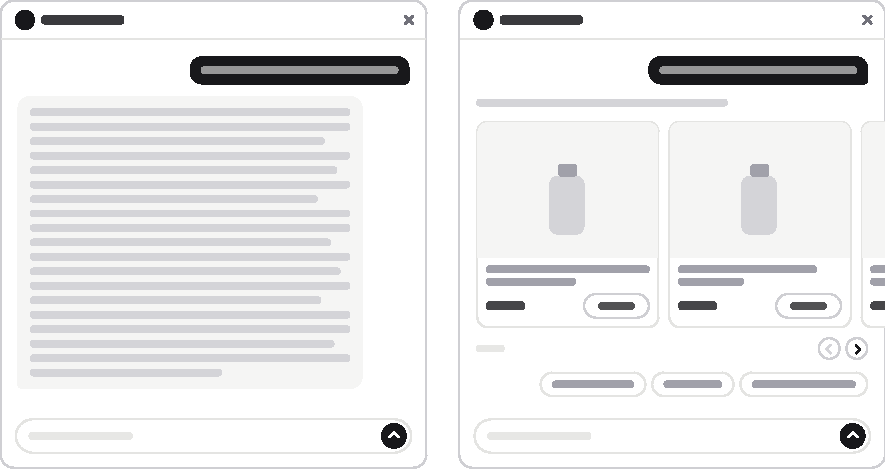
\includegraphics[width=\textwidth]{figure/02-ragioni/confronto.pdf}
	\caption[Confronto tra un assistente testuale e ChatCart]{\emph{Mockup} della risposta alla
	stessa richiesta di un assistente testuale, a sinistra, e di ChatCart, a destra.}
	\label{fig:confronto}
\end{figure}

Il potenziale di un assistente efficace è misurabile. Uno studio sperimentale condotto tra il 2023
e il 2024 su una delle maggiori piattaforme internazionali di commercio
elettronico\textsuperscript{\ref{rif:studio-genai}} ha confrontato sette applicazioni dell’IA
generativa, ciascuna con un gruppo di clienti che la usava e un gruppo di controllo. L’effetto
maggiore è quello dell’assistente che risponde alle domande dei clienti prima dell’acquisto, che ha
aumentato le vendite del 16,3\%. L’aumento deriva da un numero maggiore di clienti che acquistano,
mentre il valore medio del carrello resta invariato. I clienti che traggono più vantaggio
dall’assistente sono quelli che conoscono meno la piattaforma.

Le soluzioni disponibili sul mercato appartengono a cinque tipi, e ciascuno lascia scoperta una
parte del problema:

\begin{itemize}
	\item \textbf{Gli assistenti generici per l’assistenza clienti} risolvono richieste di supporto
	su più canali a partire dai documenti dell’azienda. Conoscono poco il catalogo e rispondono con
	testo, quindi sono adatti alla gestione di un reso più che alla scelta di un prodotto.
	\item \textbf{Gli assistenti alla vendita preconfezionati} si installano nel negozio e
	consigliano prodotti. L’interfaccia, il modello e il comportamento sono decisi dal fornitore e
	restano uguali per tutti i negozi che li adottano.
	\item \textbf{Sidekick}\textsuperscript{\ref{rif:sidekick}}, l’assistente che Shopify integra nel
	pannello di amministrazione, supporta il commerciante nella gestione del negozio e non si
	rivolge a chi acquista.
	\item \textbf{Il \emph{server} MCP del negozio}\textsuperscript{\ref{rif:storefront-mcp}}, che
	Shopify attiva per ogni negozio, espone agli agenti la ricerca nel catalogo, il carrello e le
	condizioni di vendita. È un componente destinato a chi sviluppa un agente, perché fornisce dati
	e operazioni senza un’interfaccia, e la sua ricerca è la stessa per ogni catalogo.
	\item \textbf{\gloss{ucp}{UCP}}\textsuperscript{\ref{rif:ucp}}, uno standard aperto che Shopify
	e Google hanno pubblicato nel gennaio 2026, permette a un agente di scoprire che cosa offre un
	negozio e di completare un acquisto. È pensato per gli assistenti di terze parti, per cui la
	conversazione avviene fuori dal negozio, in un’interfaccia che il marchio non controlla.
\end{itemize}

Nessuna di queste soluzioni soddisfa insieme i tre requisiti a cui i clienti di Halue attribuiscono
più valore, cioè l’identità visiva del marchio, i dati specifici del suo catalogo e un’esperienza
d’acquisto che si svolge interamente nel negozio. Un prodotto preconfezionato deve adattarsi a
tutti i commercianti, e per questo lascia poco spazio alla personalizzazione. Halue costruisce
soluzioni per il singolo cliente, perciò ha scelto di esplorare un assistente su misura basato su
un’\gloss{interfaccia-generativa}{interfaccia generativa}, in cui l’agente risponde con testo
oppure sceglie un componente da una libreria predefinita, come una scheda prodotto, e lo popola in
tempo reale con i dati del negozio. Il marchio conserva il controllo sull’aspetto dei componenti,
e il modello decide soltanto quale mostrare e con quali dati.


% !TeX root = ../../tesi.tex

\section{Il commercio agentico nella visione di Halue}
\label{sec:commercio-agentico}

Il \gloss{commercio-agentico}{commercio agentico} è l’insieme delle esperienze d’acquisto in cui un
agente di intelligenza artificiale accompagna il cliente nella ricerca, nella scelta e
nell’acquisto di un prodotto. Si sta sviluppando in due direzioni:

\begin{itemize}
	\item il negozio si apre ad assistenti generici di terze parti, che lo raggiungono con protocolli
	come MCP e UCP, e il cliente conversa altrove mentre il negozio fornisce catalogo e pagamento;
	\item l’assistente appartiene al marchio e opera all’interno del negozio, con la sua interfaccia
	e con strumenti scritti per il suo catalogo.
\end{itemize}

Le piattaforme promuovono la prima direzione, che un commerciante può adottare senza alcuno
sviluppo dedicato. La seconda richiede un progetto su misura, ed è quella in cui un’azienda come
Halue può offrire un servizio ai propri clienti. ChatCart la esplora.

Prima dello \emph{stage} Halue disponeva già di alcune premesse, cioè i negozi realizzati per
marchi che vendono su più mercati e gli agenti collegati ai dati dei negozi con strumenti propri
(\secref{sec:innovazione}). Non aveva invece esperienza su un assistente rivolto al cliente finale,
che pone problemi diversi da quelli di un agente a uso interno perché deve integrarsi con il tema
del negozio, rispondere in pochi secondi e comportarsi in modo prevedibile con qualsiasi
interlocutore. Lo \emph{stage} aveva lo scopo di costruire questa competenza su un caso
sufficientemente circoscritto da poter essere completato nella durata prevista.

Al termine dello \emph{stage}, il risultato costituisce per l’azienda una base di ricerca e
sviluppo. L’obiettivo dichiarato è arrivare a proporre questo tipo di soluzione ai clienti come
servizio, con tempi e forma ancora da stabilire. Il primo passo è stata la presentazione al
\emph{team} del 9 novembre 2026, l’ultimo giorno di \emph{stage}, articolata in trenta minuti
dedicati al prodotto, quindici alla parte tecnica e quindici alle domande. Le domande hanno
mostrato quali aspetti interessano a chi riprenderà il lavoro, in particolare le scelte di
progettazione, come la gestione dello stato nella sincronizzazione del carrello, e il modo in cui
ho istruito l’agente perché si comportasse come previsto.


% !TeX root = ../../tesi.tex

\section{Obiettivi e vincoli del progetto}
\label{sec:obiettivi}

Mi sono candidato a luglio 2026 e ad agosto ho sostenuto un colloquio conoscitivo con il
\emph{tutor} e con il fondatore. Halue mi ha poi proposto due temi, l’interfaccia generativa e la
gestione del contesto di un agente. Ho scelto il primo e ho proposto di declinarlo in un assistente
che seleziona e popola componenti dell’interfaccia con i dati del negozio.

Il piano organizza il prototipo su due livelli (\figref{fig:livelli}). L’\emph{app layer} è il
\emph{widget} di chat nel negozio e si limita a visualizzare la conversazione e i componenti.
L’\emph{agent layer} è il \emph{backend} che ospita l’agente e conserva lo stato della
conversazione. Per interrogare le API di Shopify l’agente usa il
\gloss{tool-calling}{\emph{tool calling}}, il meccanismo con cui un modello linguistico chiede al
programma che lo ospita di eseguire una funzione e ne riceve il risultato.

\begin{figure}[htbp]
	\centering
	\setstretch{1}
	% L'architettura su due livelli prevista dal piano di lavoro: il widget nel negozio
% (app layer) e il backend che ospita l'agente (agent layer), con i servizi esterni a destra.
% Il disegno è largo quanto il testo (150 mm): si include con \input, senza ridimensionarlo.

\begin{tikzpicture}[
	every node/.style={text=FiguraTesto},
	blocco/.style={draw=FiguraTenue, fill=white, rounded corners=3pt, text width=#1-2mm,
		minimum width=#1, minimum height=13mm, align=center, inner sep=1.5pt,
		font=\fontsize{7.5}{9}\selectfont,
		execute at begin node={\hyphenpenalty=10000\exhyphenpenalty=10000}},
	blocco/.default=32mm,
	etichetta/.style={font=\fontsize{7}{8.5}\selectfont, text=FiguraTenue, inner sep=1pt,
		align=center},
]
	\begin{scope}[on background layer]
		\path[partizione] (0mm, 0mm) rectangle (38mm, -44mm);
		\path[intestazione] (0mm, 0mm) rectangle (38mm, -6mm);
		\node[titolo] at (19mm, -3mm) {\emph{App layer}: negozio};
		\path[partizione] (72mm, 0mm) rectangle (110mm, -44mm);
		\path[intestazione] (72mm, 0mm) rectangle (110mm, -6mm);
		\node[titolo] at (91mm, -3mm) {\emph{Agent layer}: \emph{backend}};
		\path[partizione] (122mm, 0mm) rectangle (150mm, -44mm);
		\path[intestazione] (122mm, 0mm) rectangle (150mm, -6mm);
		\node[titolo] at (136mm, -3mm) {Servizi esterni};
	\end{scope}

	\node[blocco] (widget) at (19mm, -16mm)
		{\voce{\emph{Widget} di chat}{mostra la conversazione}};
	\node[blocco] (componenti) at (19mm, -34mm)
		{\voce{Libreria di componenti}{popolati con i dati del negozio}};
	\node[blocco] (agente) at (91mm, -16mm)
		{\voce{Agente}{sceglie testo o componente, esegue gli strumenti}};
	\node[blocco] (stato) at (91mm, -34mm)
		{\voce{Stato}{storico della conversazione}};
	\node[blocco=24mm] (llm) at (136mm, -16mm) {\voce{Modello linguistico}{genera le risposte}};
	\node[blocco=24mm] (api) at (136mm, -34mm) {\voce{API di Shopify}{catalogo, carrello, ordini}};

	\draw[freccia] ([yshift=3mm]widget.east) -- node[etichetta, above=0.5mm]
		{messaggio del cliente} ([yshift=3mm]agente.west);
	\draw[freccia] ([yshift=-3mm]agente.west) -- node[etichetta, below=0.5mm]
		{testo o componente\\e tre messaggi suggeriti} ([yshift=-3mm]widget.east);
	\draw[freccia] (widget) -- node[etichetta, right=0.5mm] {disegna} (componenti);
	\draw[freccia, {Stealth[length=1.8mm,width=1.4mm]}-{Stealth[length=1.8mm,width=1.4mm]}]
		(agente) -- (stato);
	\draw[freccia, {Stealth[length=1.8mm,width=1.4mm]}-{Stealth[length=1.8mm,width=1.4mm]}]
		(agente.east) -- (llm.west);
	\draw[freccia] (agente.east) ++(0, -3mm) -- ++(6mm, 0) |- (api.west);
\end{tikzpicture}

	\caption[L’architettura su due livelli prevista dal piano di lavoro]{L’architettura su due
	livelli prevista dal piano di lavoro. Il \emph{widget} non contiene logica conversazionale: ogni
	decisione spetta all’agente, che può interrogare più volte modello e API prima di rispondere.}
	\label{fig:livelli}
\end{figure}

Gli obiettivi hanno un identificativo, che uso nel resto della relazione, e tre livelli di
priorità. Gli obiettivi obbligatori (\tabref{tbl:obbligatori}) sono vincolanti e, oltre a
dimostrare la fattibilità dell’approccio, chiedono di misurarne l’efficacia.

Gli obiettivi desiderabili hanno un valore aggiunto riconoscibile, quelli facoltativi un valore
aggiunto non prioritario (\tabref{tbl:desiderabili}). Riprendono tre aspetti che il \emph{tutor}
ha indicato come interessanti per l’azienda: il supporto a più mercati, i temi Hydrogen, in cui il
riuso dei componenti React è più semplice e l’integrazione con il carrello più complessa, e una
ricerca nel catalogo scritta su misura, perché il \emph{tutor} giudicava elementare quella del
\emph{server} MCP di Shopify.

\begin{tabellatesi}{P{0.1}P{0.9}}
	{Gli obiettivi obbligatori del piano di lavoro.}
	{tbl:obbligatori}
	\toprule
	\rowcolor{TabellaIntestazione} \textbf{ID} & \textbf{Obiettivo} \\
	\midrule
	OB1 & \emph{App layer}: \emph{widget} di chat in React e TypeScript integrato nel negozio \\
	OB2 & \emph{Agent layer}: \emph{backend} Node.js con un agente dotato di \emph{tool calling}, in
	grado di interrogare le API di Shopify \\
	OB3 & Risposte in linguaggio naturale (domande generali, sui prodotti, di chiarimento) oppure con
	un componente predefinito, scelto e popolato in base alla conversazione \\
	OB4 & Libreria di almeno due o tre componenti flessibili e tre messaggi suggeriti per ogni
	risposta \\
	OB5 & Raccolta di metriche di coinvolgimento e di conversione sull’uso del \emph{widget} \\
	\bottomrule
\end{tabellatesi}

\begin{tabellatesi}{P{0.1}P{0.2}P{0.7}}
	{Gli obiettivi desiderabili e facoltativi del piano di lavoro.}
	{tbl:desiderabili}
	\toprule
	\rowcolor{TabellaIntestazione} \textbf{ID} & \textbf{Priorità} & \textbf{Obiettivo} \\
	\midrule
	DE1 & desiderabile & Supporto a \gloss{shopify-markets}{Shopify Markets}, la funzione con cui un
	negozio vende in più paesi con lingue e valute diverse \\
	DE2 & desiderabile & Componente per lo stato dell’ordine e il supporto dopo la vendita \\
	FA1 & facoltativo & Prova di fattibilità dell’integrazione su Hydrogen, con il riuso dei
	componenti del \emph{widget} \\
	FA2 & facoltativo & Confronto sperimentale tra la ricerca su misura, il \emph{server} MCP di
	Shopify e un eventuale \emph{server} MCP proprio \\
	\bottomrule
\end{tabellatesi}

Il piano ripartisce 310 ore indicative tra dieci attività (\figref{fig:piano}) e prevede che la
ripartizione sia rifinita con il \emph{tutor} nelle prime settimane. Nel capitolo 3 la confronto
con l’uso effettivo del tempo.

\begin{figure}[htbp]
	\centering
	\setstretch{1}
	% La ripartizione indicativa delle 310 ore prevista dal piano di lavoro, come grafico a torta.
% Le fette seguono l'ordine del piano in senso orario dall'alto: in grigio chiaro le attività che
% precedono il codice, in bordeaux lo sviluppo dei due livelli, in grigio medio quelle successive.
% Il disegno è largo quanto il testo (150 mm): si include con \input, senza ridimensionarlo.

\begin{tikzpicture}[every node/.style={text=FiguraTesto}]
	\def\raggio{22mm}
	\def\inizio{90}
	% ore/colore/lato (1 a destra, -1 a sinistra)/quota dell'etichetta/titolo/dettaglio
	\foreach \ore/\colore/\lato/\quota/\titolo/\dettaglio in {
		20/TabellaIntestazione/1/27/{Studio}/{Shopify e strumenti per agenti},
		20/TabellaIntestazione/1/16/{Analisi dei requisiti}/{e perimetro del progetto},
		20/TabellaIntestazione/1/5/{Progettazione}/{dell’architettura},
		40/TabellaIntestazione/1/-7/{Negozio di sviluppo}/{e accesso ai dati},
		50/FiguraAccento/1/-21/{\emph{Agent layer}}/{sviluppo del \emph{backend}},
		60/FiguraAccento!65/-1/-21/{\emph{App layer}}/{sviluppo del \emph{widget}},
		30/FiguraBordo/-1/-7/{Integrazione}/{del flusso conversazionale},
		30/FiguraBordo/-1/5/{Metriche}/{raccolta dei dati di utilizzo},
		20/FiguraBordo/-1/16/{\emph{Test}}/{flusso utente e casi limite},
		20/FiguraBordo/-1/27/{Documentazione}/{tecnica}} {
		\pgfmathsetmacro\fine{\inizio - \ore/310*360}
		\pgfmathsetmacro\medio{(\inizio + \fine)/2}
		\fill[\colore, draw=white, line width=0.8pt] (0, 0) -- (\inizio:\raggio)
			arc[start angle=\inizio, end angle=\fine, radius=\raggio] -- cycle;
		\draw[FiguraTenue] (\medio:\raggio + 1mm) -- (\lato*\raggio + \lato*10mm, \quota mm)
			-- ++(\lato*3mm, 0);
		\ifnum\lato=1
			\node[anchor=west, align=left, font=\fontsize{7.5}{9}\selectfont]
				at (\raggio + 14mm, \quota mm) {\voce{\titolo, \ore{} ore}{\dettaglio}};
		\else
			\node[anchor=east, align=right, font=\fontsize{7.5}{9}\selectfont]
				at (-\raggio - 14mm, \quota mm) {\voce{\titolo, \ore{} ore}{\dettaglio}};
		\fi
		\global\let\inizio\fine
	}
\end{tikzpicture}

	\caption[La ripartizione delle ore prevista dal piano di lavoro]{La ripartizione delle ore
	prevista dal piano di lavoro, in senso orario dall’alto. In grigio chiaro le attività che
	precedono la scrittura del codice, in bordeaux lo sviluppo dei due livelli, in grigio medio le
	attività che lo completano.}
	\label{fig:piano}
\end{figure}

Per l’azienda il criterio di successo era un prototipo funzionante dall’inizio alla fine su un
negozio di esempio, accompagnato da una valutazione onesta di ciò che funziona e di ciò che non
funziona. Valuto il grado di soddisfacimento di ogni obiettivo nella \secref{sec:soddisfacimento}.

Il progetto aveva i seguenti vincoli:

\begin{itemize}
	\item \textbf{Quantità di lavoro}: da 300 a 320 ore, con una distribuzione al massimo a tempo
	pieno, dal 14 settembre al 9 novembre 2026.
	\item \textbf{Luogo di lavoro}: da remoto, con un giorno a settimana in sede, un allineamento
	quotidiano con il \emph{tutor} e una riunione settimanale di un’ora.
	\item \textbf{Tecnologie}: TypeScript in tutto il progetto. Il piano rimandava alle prime settimane la scelta degli strumenti
	per costruire l’agente e del modello linguistico, che il \emph{tutor} ha lasciato a me.
	\item \textbf{Piattaforma}: prima i temi Liquid, che sono i più diffusi, e Hydrogen soltanto come
	eventuale approfondimento finale.
	\item \textbf{Ambiente}: un unico negozio di sviluppo, senza clienti né traffico reali, con due
	temi installati per le prove. L’ho allestito come un negozio di cosmetica botanica con circa
	quaranta prodotti, perché il comportamento di un assistente dipende dal catalogo su cui opera, e
	varianti, collezioni, confezioni regalo, prodotti esauriti e archiviati lo avvicinano a un caso
	reale.
	\item \textbf{Natura del prodotto}: un prototipo di ricerca e sviluppo, essenziale ma solido,
	senza i requisiti di scala e di costo di un prodotto in produzione.
\end{itemize}


% !TeX root = ../../tesi.tex

\section{Motivazioni e obiettivi personali}
\label{sec:obiettivi-personali}

Da marzo 2026 lavoro in proprio come sviluppatore di negozi Shopify, occupandomi di migrazioni da
altre piattaforme, gestione dei negozi e automazioni. La mia esperienza riguardava però soltanto i
temi Liquid e non lo sviluppo di applicazioni. Tra le proposte di \emph{stage}, quella di Halue
riguardava progetti su Shopify, era la più vicina al mio lavoro e mi offriva ciò che mi mancava:
lo sviluppo di un’applicazione in un’azienda che lavora su questa piattaforma ogni giorno. Per
questo l’ho scelta.

L’idea dell’interfaccia generativa è di Halue. Quando l’azienda me l’ha proposta vi ho riconosciuto
l’esigenza di un mio cliente, che mi aveva parlato di un assistente capace di dare assistenza ai
visitatori del suo negozio e di indirizzarli verso l’acquisto. Il progetto aveva quindi per me un
valore che andava oltre lo \emph{stage}, e questo ha orientato sia la scelta del tema sia la
proposta dei componenti.

Da queste ragioni ho ricavato quattro obiettivi personali (\tabref{tbl:personali}), che valuto
insieme a quelli del piano nella \secref{sec:soddisfacimento}.

\begin{tabellatesi}{P{0.1}P{0.9}}
	{I miei obiettivi personali per lo \emph{stage}.}
	{tbl:personali}
	\toprule
	\rowcolor{TabellaIntestazione} \textbf{ID} & \textbf{Obiettivo} \\
	\midrule
	OP1 & Estendere le mie competenze su Shopify dai temi allo sviluppo di applicazioni \\
	OP2 & Acquisire esperienza nella progettazione di sistemi basati su agenti \\
	OP3 & Ricavare dal progetto conoscenze e soluzioni riutilizzabili nella mia attività
	professionale \\
	OP4 & Gestire in autonomia il lavoro da remoto, dove nessuno segue la mia giornata in modo
	continuo e spetta a me organizzarla, stabilire le priorità e prevedere le pause \\
	\bottomrule
\end{tabellatesi}

% DA CONFERMARE: il cliente resta anonimo finché non autorizza la citazione del nome.

